\documentclass[11pt]{article}
\usepackage{graphicx}
\usepackage{listings}
\usepackage{algorithm}
\usepackage{algorithmic}
\usepackage[english]{babel}
\usepackage{amsmath}
\usepackage{latexsym}
\usepackage{amsfonts}
\usepackage[normalem]{ulem}
\usepackage{array}
\usepackage{amssymb}
\usepackage{subfig}
\usepackage{wrapfig}
\usepackage{wasysym}
\usepackage{enumitem}
\setlist[itemize]{after=\vspace{-0.50\baselineskip},before=\vspace{-0.95\baselineskip}}
\newlist{ucmenum}{enumerate}{1}
\setlist[ucmenum]{label=\arabic*,after=\vspace{-0.50\baselineskip},before=\vspace{-0.95\baselineskip}}
\usepackage{adjustbox}
\usepackage{ragged2e}
\usepackage{hhline}
\usepackage[svgnames,table]{xcolor}
\usepackage{tikz}
\usepackage{longtable}
\usepackage{changepage}
\usepackage{setspace}
\usepackage{multicol}
\usepackage{tabto}
\usepackage{float}
\usepackage{multirow}
\usepackage{makecell}
\usepackage{fancyhdr}
\usepackage[toc,page]{appendix}
\usepackage[utf8]{inputenc}
\usepackage{flowchart}
\usepackage[colorlinks]{hyperref}
\usepackage{glossaries}
\usepackage{apacite}
\usepackage{color}
\makeglossaries

\newacronym{cyclomaticnumber}{Cyclomatic Number}{Software metric, used to indicate the complexity of a program}
\newacronym{gqm}{GQM}{Goal Question Metric}
\newacronym{sis}{SIS}{Student Information System}
\newacronym{wmc}{WMC}{Weighted Methods per Class}
\newacronym{cf}{CF}{Coupling Factor}
\newacronym{lcom}{LCOM*}{Lack of Cohesion in Methods}
\newacronym{sloc}{SLOC}{Source Line of Code}
\newacronym{cloc}{CLOC}{Count Lines of Code}
\newacronym{ucm}{UCM}{Use Case Model}
\newacronym{ucp}{UCP}{Use Case Points}
\newacronym{uucp}{UUCP}{Unadjusted Use Case Points}
\newacronym{uucw}{UUCW}{Unadjusted Use Case Weight}
\newacronym{uaw}{UAW}{Unadjusted Actor Weight}
\newacronym{tcf}{TCF}{Technical Complexity Factor}
\newacronym{ecf}{ECF}{Environment Complexity Factor}
\newacronym{pf}{PF}{Productivity Factor}
\newacronym{wti}{WTi}{Technical Complexity Factor Weight}
\newacronym{fi}{Fi}{Perceived Impact Factor}
\newacronym{wei}{WEi}{Environmental Complexity Factor Weight}
\newacronym{cocomo}{COCOMO}{Constructive Cost Model}
\newacronym{kdsi}{KDSI}{Kilo Delivered Source Instructions}
\newacronym{sd}{SD}{Standard deviation}

\newglossaryentry{radix}{
	name=Radix sort,
    description={A sorting algorithm that gives each item a unique identifier and distributes each of them to a bucket. After each pass, items are being sorted based on the value of the unique identifier. \cite{nist}}
}
\newglossaryentry{integration}
{
  name=Integration tests,
  description={tests performed to detect defaults in the interation between integrated components or systems}
}

\glsaddall

\hypersetup{pdfborder={0 0 0},
colorlinks=true,
breaklinks=true,
urlcolor=blue,
linkcolor=black,
citecolor=blue}

\setlength{\parindent}{0in}

\definecolor{dkgreen}{rgb}{0,0.6,0}
\definecolor{gray}{rgb}{0.5,0.5,0.5}
\definecolor{mauve}{rgb}{0.58,0,0.82}

\lstset{frame=tb,
  language=R,
  aboveskip=3mm,
  belowskip=3mm,
  showstringspaces=false,
  columns=flexible,
  basicstyle={\small\ttfamily},
  numbers=left,
  numberstyle=\tiny\color{gray},
  keywordstyle=\color{blue},
  commentstyle=\color{dkgreen},
  stringstyle=\color{mauve},
  breaklines=true,
  breakatwhitespace=true,
  tabsize=3
}

\makeatletter
\renewcommand\paragraph{\@startsection{paragraph}{4}{\z@}%
            {-2.5ex\@plus -1ex \@minus -.25ex}%
            {1.25ex \@plus .25ex}%
            {\normalfont\normalsize\bfseries}}
\makeatother
\setcounter{secnumdepth}{4} % how many sectioning levels to assign numbers to
\setcounter{tocdepth}{4}    % how many sectioning levels to show in ToC

\begin{document}
\title{Software Measurement (SOEN6611)\\Summer 2018\\Descriptive Statistics\\Team J\\Deliverable 1}
\author{Ksenia Popova, Farhan Shaheen, Himalaya Yadav Reddiboina,\\Kaushik Samanta, Adrien Poupa, Yousef Saatchi Tabriz}
\date{}
\maketitle

\newpage

\tableofcontents

\newpage
\section{Goal-Question-Metric}

\subsection{Goal}

To create a subsystem, integrated in a \gls{sis} in order to be used to collect statistics about students grades. The subsystem is named "Descriptive Statistics". The subsystem must be accessible by the \gls{sis} and usable by the students, administration and the professors. Descriptive Statistics has to provide students statistics of their grades in an easy manner. Professors must be able to enter the grades and see the students' statistics quickly. The administrators must be able to oversee the system without any hassle. Descriptive Statistics must be able to recover from errors.
\newline
\newline
Note: in this document, "users" designate the actors of Descriptive Statistics; professors, students and a department member.

\subsection{Question-Metric}


    
\begin{enumerate}
\item
   \begin{enumerate}
	\item Question: How to ensure that the Descriptive Statistics is connected to the \gls{sis}?
    \item Metric: Create \gls{integration} and assess their success to evaluate the connection between Descriptive Statistics and the \gls{sis}. This is an objective metric, based on the viewpoint on the subsystem.
    \item Mechanism:
    \begin{enumerate}
    \item Owner = Lead Developer
    \item Frequency Collected = Following Each Major Software Release
    \item Frequency Reported = Quarterly
    \end{enumerate}
\end{enumerate}
\item
    \begin{enumerate}
    \item Question: How to ensure the system is easy to use by the students?
    \item Metric: Conduct a survey using the System Usability Scale \cite{mifsud}. This is a subjective metric, based on the viewpoint of the users.
    \item Mechanism:
	\begin{enumerate}
    \item Owner = Product Manager
    \item Frequency Collected = Following The End of the First Session
    \item Frequency Reported = Quarterly
    \end{enumerate}
\end{enumerate}
\item
	\begin{enumerate}
    \item Question: How to ensure the system is easy to use by the professors?
    \item Metric: Conduct a survey using the Computer System Usability \cite{mifsud}. This is a subjective metric, based on the viewpoint of the users.
    \item Mechanism:
	\begin{enumerate}
    \item Owner = Product Manager
    \item Frequency Collected = Following The End of the First Session
    \item Frequency Reported = Quarterly
    \end{enumerate}
\end{enumerate}
\item
	\begin{enumerate}
    \item Question: How to ensure the system is easy to use by the department?
    \item Metric: Conduct a survey using the Computer System Usability \cite{mifsud} at the end of the first session. This is a subjective metric, based on the viewpoint of the users.
    \item Mechanism:
	\begin{enumerate}
    \item Owner = Product Manager
    \item Frequency Collected = Following The End of the First Session
    \item Frequency Reported = Quarterly
    \end{enumerate}
\end{enumerate}
\item
	\begin{enumerate}
    \item Question: How to ensure that a professor can enter a grade in Descriptive Statistics in no more than 5 seconds?
    \item Metric: Calculate the Time-Based Efficiency \cite{mifsud}. This is an objective metric, based on the viewpoint on the subsystem.
    \item Mechanism:
	\begin{enumerate}
    \item Owner = Lead Developer
    \item Frequency Collected = Every Day
    \item Frequency Reported = Quarterly
    \end{enumerate}
\end{enumerate}
\item
	\begin{enumerate}
    \item Question: How to ensure that professors, students and department does not give up on using Descriptive Statistics?
    \item Metric: Calculate the Completion Rate \cite{sauro2}. This is an objective metric, based on the viewpoint on the subsystem.
    \item Mechanism:
	\begin{enumerate}
    \item Owner = Product Manager
    \item Frequency Collected = Every Day
    \item Frequency Reported = Quarterly
    \end{enumerate}
\end{enumerate}
\item
	\begin{enumerate}
    \item Question: How to prevent errors in Descriptive Statistics?
    \item Metric: Record every error encountered by users in Descriptive Statistics \cite{seeley}. This is an objective metric, based on the viewpoint on the subsystem.
    \item Mechanism:
	\begin{enumerate}
    \item Owner = Lead Developer
    \item Frequency Collected = Every Day
    \item Frequency Reported = Quarterly
    \end{enumerate}
\end{enumerate}
\item
	\begin{enumerate}
    \item Question: How to ensure that Descriptive Statistics meet students', professors' and department's expectations?
    \item Metric: Use the Single Ease Question metric \cite{mifsud} before and after a task to see the difference. in terms of expectations. This is a subjective metric, based on the viewpoint of the users.
    \item Mechanism:
	\begin{enumerate}
    \item Owner = Product Manager
    \item Frequency Collected = Before and After Every Task
    \item Frequency Reported = Quarterly
    \end{enumerate}
\end{enumerate}
\item
	\begin{enumerate}
    \item Question: How to ensure that Descriptive Statistics does not take more than one second for a calculation to complete?
    \item Metric: Log Load Time \cite{west}. This is an objective metric, based on the viewpoint on the subsystem.
    \item Mechanism:
	\begin{enumerate}
    \item Owner = Lead Developer
    \item Frequency Collected = Every Day
    \item Frequency Reported = Quarterly
    \end{enumerate}
\end{enumerate}
\item
	\begin{enumerate}
    \item Question: How to make sure that users are able to use the system autonomously?
    \item Metric: Record the Frequency of help and documentation use. This is an objective metric, based on the viewpoint on the subsystem and the support staff.
    \item Mechanism:
	\begin{enumerate}
    \item Owner = Product Manager
    \item Frequency Collected = Every Day
    \item Frequency Reported = Quarterly
    \end{enumerate}
\end{enumerate}
\item
	\begin{enumerate}
    \item Question: How many clicks does Descriptive Statistics require to complete the tasks?
    \item Metric: Record the Number of Clicks \cite{kelkar}. This is an objective metric, based on the viewpoint on the subsystem.
    \item Mechanism:
	\begin{enumerate}
    \item Owner = Product Manager
    \item Frequency Collected = Every Day
    \item Frequency Reported = Quarterly
    \end{enumerate}
\end{enumerate}
\item
	\begin{enumerate}
    \item Question: How to make sure that the learning curve of Descriptive Statistics is smooth?
    \item Metric: Compare the Time-Based Efficiency \cite{mifsud} for a first time user and a returning user. This is an objective metric, based on the viewpoint on the subsystem.
    \item Mechanism:
	\begin{enumerate}
    \item Owner = Product Manager
    \item Frequency Collected = Every Day
    \item Frequency Reported = Quarterly
    \end{enumerate}
\end{enumerate}
\end{enumerate}

\newpage
\section{Use Case Model}

\subsection{Use Case Diagram}

\begin{figure}[h!]
	\centering
		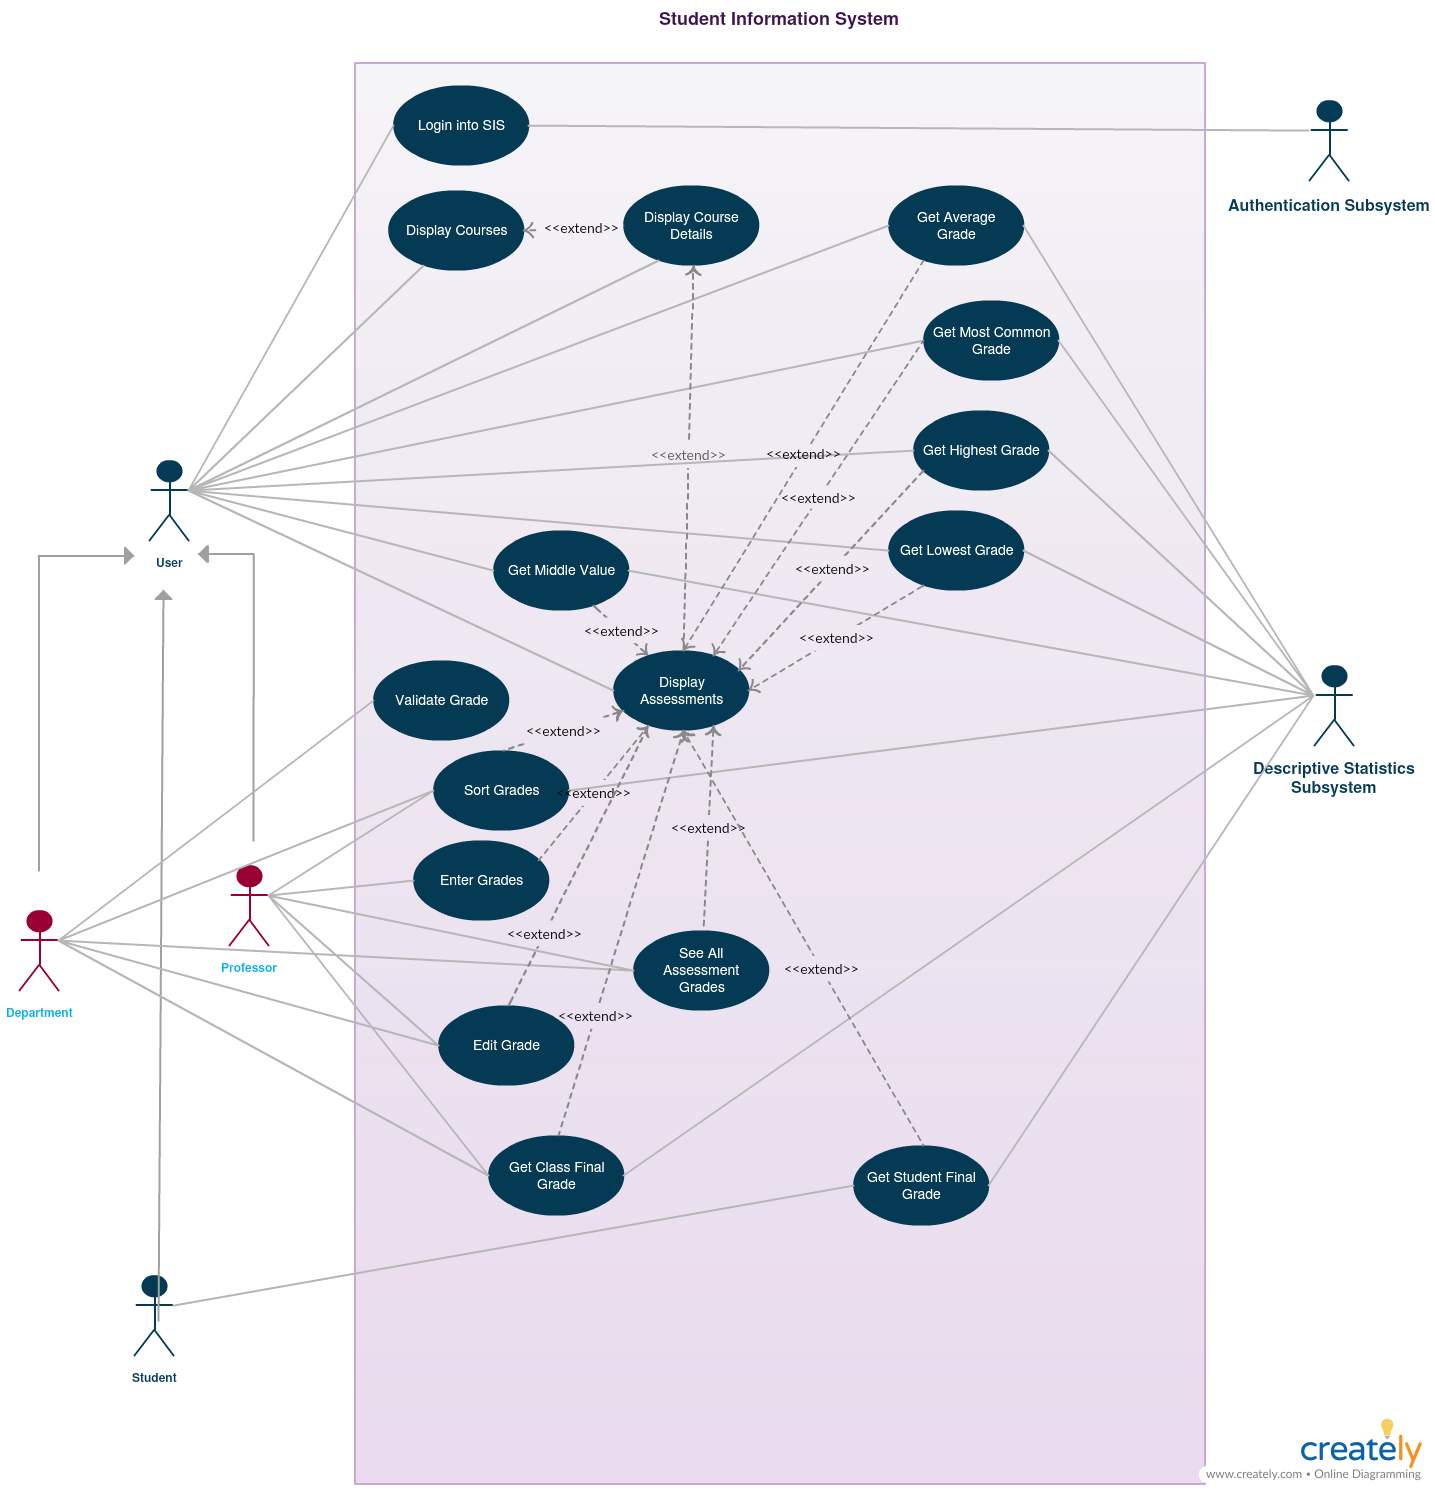
\includegraphics[width=\textwidth]{usecasediagram.png}
	\caption{Use Case Model}
	\label{fig:usecasemodel}
\end{figure}

\subsection{Use Cases}

%%%%%%%%%%%%%%%%%%%% Table No: 1 starts here %%%%%%%%%%%%%%%%%%%%


\begin{table}[H]
 			\centering
\begin{tabular}{p{1.23in}p{4.87in}}
\hline
%row no:1
\multicolumn{1}{|p{1.23in}}{Use Case ID} & 
\multicolumn{1}{|p{4.87in}|}{UC-1} \\
\hhline{--}
%row no:2
\multicolumn{1}{|p{1.23in}}{Use Case Name} & 
\multicolumn{1}{|p{4.87in}|}{Log in to the System} \\
\hhline{--}
%row no:3
\multicolumn{1}{|p{1.23in}}{Primary Actors} & 
\multicolumn{1}{|p{4.87in}|}{\begin{itemize}
	\item Department \par 	\item Professor \par 	\item Student
\end{itemize}} \\
\hhline{--}
%row no:4
\multicolumn{1}{|p{1.23in}}{Secondary Actor} & 
\multicolumn{1}{|p{4.87in}|}{Authentication Subsystem} \\
\hhline{--}
%row no:5
\multicolumn{1}{|p{1.23in}}{Priority} & 
\multicolumn{1}{|p{4.87in}|}{High} \\
\hhline{--}
%row no:6
\multicolumn{1}{|p{1.23in}}{Description} & 
\multicolumn{1}{|p{4.87in}|}{User can login into the System.} \\
\hhline{--}
%row no:7
\multicolumn{1}{|p{1.23in}}{Pre-conditions} & 
\multicolumn{1}{|p{4.87in}|}{\begin{itemize}
	\item User has a valid account.
\end{itemize}} \\
\hhline{--}
%row no:8
\multicolumn{1}{|p{1.23in}}{Post-conditions} & 
\multicolumn{1}{|p{4.87in}|}{\begin{itemize}
	\item User logged in.
\end{itemize}} \\
\hhline{--}
%row no:9
\multicolumn{1}{|p{1.23in}}{Normal Flow} & 
\multicolumn{1}{|p{4.87in}|}{\begin{ucmenum}
	\item User requests the login page of the system. \par 	\item System displays the login page. \par 	\item User enters their username and their password. \par 	\item User clicks on $``$Login$"$ . \par 	\item System checks the User’s credentials. \par 	\item System redirects User to the homepage. \par 	\item System displays the homepage. \par 	\item User sees the homepage.
\end{ucmenum}} \\
\hhline{--}
%row no:10
\multicolumn{1}{|p{1.23in}}{Alternate Flow} & 
\multicolumn{1}{|p{4.87in}|}{\ \ \ \ \  5. a. Credentials provided by the User were invalid.} \\
\hhline{--}

\end{tabular}
 \end{table}


%%%%%%%%%%%%%%%%%%%% Table No: 1 ends here %%%%%%%%%%%%%%%%%%%%



 %%%%%%%%%%%%  Starting New Page here %%%%%%%%%%%%%%

\newpage

\vspace{\baselineskip}

%%%%%%%%%%%%%%%%%%%% Table No: 2 starts here %%%%%%%%%%%%%%%%%%%%


\begin{table}[H]
 			\centering
\begin{tabular}{p{1.23in}p{4.87in}}
\hline
%row no:1
\multicolumn{1}{|p{1.23in}}{Use Case ID} & 
\multicolumn{1}{|p{4.87in}|}{UC-2} \\
\hhline{--}
%row no:2
\multicolumn{1}{|p{1.23in}}{Use Case Name} & 
\multicolumn{1}{|p{4.87in}|}{Display Courses} \\
\hhline{--}
%row no:3
\multicolumn{1}{|p{1.23in}}{Primary Actors} & 
\multicolumn{1}{|p{4.87in}|}{\begin{itemize}
	\item Department \par 	\item Professor \par 	\item Student
\end{itemize}} \\
\hhline{--}
%row no:4
\multicolumn{1}{|p{1.23in}}{Secondary Actor} & 
\multicolumn{1}{|p{4.87in}|}{None} \\
\hhline{--}
%row no:5
\multicolumn{1}{|p{1.23in}}{Priority} & 
\multicolumn{1}{|p{4.87in}|}{High} \\
\hhline{--}
%row no:6
\multicolumn{1}{|p{1.23in}}{Description} & 
\multicolumn{1}{|p{4.87in}|}{User can display a list of their courses.} \\
\hhline{--}
%row no:7
\multicolumn{1}{|p{1.23in}}{Pre-conditions} & 
\multicolumn{1}{|p{4.87in}|}{\begin{itemize}
	\item User is logged in to the System.
\end{itemize}} \\
\hhline{--}
%row no:8
\multicolumn{1}{|p{1.23in}}{Post-conditions} & 
\multicolumn{1}{|p{4.87in}|}{\begin{itemize}
	\item A list of courses were displayed.
\end{itemize}} \\
\hhline{--}
%row no:9
\multicolumn{1}{|p{1.23in}}{Normal Flow} & 
\multicolumn{1}{|p{4.87in}|}{\begin{ucmenum}
	\item User requests the list of the courses available. \par 	\item The System displays the list of the courses available: \par 	\item If the user is a Professor: list of courses taught by the Professor. \par 	\item If the user is a Department member: list of the courses that the Department offers. \par 	\item If the user is a Student: list of courses that the Student is enrolled in.
\end{ucmenum}} \\
\hhline{--}
%row no:10
\multicolumn{1}{|p{1.23in}}{Alternate Flow} & 
\multicolumn{1}{|p{4.87in}|}{\ \ \ \ \  2. a. Professor is teaching a course but does not have access to the course. \par \ \ \ \ \  2. b. Department offers a course but does not have access to the course. \par \ \ \ \ \  2. c. Student is enrolled in a course but does not have access to the course.} \\
\hhline{--}

\end{tabular}
 \end{table}


%%%%%%%%%%%%%%%%%%%% Table No: 2 ends here %%%%%%%%%%%%%%%%%%%%



 %%%%%%%%%%%%  Starting New Page here %%%%%%%%%%%%%%

\newpage

\vspace{\baselineskip}
\vspace{\baselineskip}


%%%%%%%%%%%%%%%%%%%% Table No: 3 starts here %%%%%%%%%%%%%%%%%%%%


\begin{table}[H]
 			\centering
\begin{tabular}{p{1.23in}p{4.87in}}
\hline
%row no:1
\multicolumn{1}{|p{1.23in}}{Use Case ID} & 
\multicolumn{1}{|p{4.87in}|}{UC-3} \\
\hhline{--}
%row no:2
\multicolumn{1}{|p{1.23in}}{Use Case Name} & 
\multicolumn{1}{|p{4.87in}|}{Display Course Details} \\
\hhline{--}
%row no:3
\multicolumn{1}{|p{1.23in}}{Primary Actors} & 
\multicolumn{1}{|p{4.87in}|}{\begin{itemize}
	\item Department \par 	\item Professor \par 	\item Student
\end{itemize}} \\
\hhline{--}
%row no:4
\multicolumn{1}{|p{1.23in}}{Secondary Actor} & 
\multicolumn{1}{|p{4.87in}|}{None} \\
\hhline{--}
%row no:5
\multicolumn{1}{|p{1.23in}}{Priority} & 
\multicolumn{1}{|p{4.87in}|}{High} \\
\hhline{--}
%row no:6
\multicolumn{1}{|p{1.23in}}{Description} & 
\multicolumn{1}{|p{4.87in}|}{User can display a list of their courses.} \\
\hhline{--}
%row no:7
\multicolumn{1}{|p{1.23in}}{Pre-conditions} & 
\multicolumn{1}{|p{4.87in}|}{\begin{itemize}
	\item User is logged in to the System. \par 	\item User requested to see course details from the course list. \par 	\item Professor has access to the course, course is contained in Department, or Student has access to the course.
\end{itemize}} \\
\hhline{--}
%row no:8
\multicolumn{1}{|p{1.23in}}{Post-conditions} & 
\multicolumn{1}{|p{4.87in}|}{\begin{itemize}
	\item A course was displayed.
\end{itemize}} \\
\hhline{--}
%row no:9
\multicolumn{1}{|p{1.23in}}{Normal Flow} & 
\multicolumn{1}{|p{4.87in}|}{\begin{ucmenum}
	\item User selects a course from the course list. \par 	\item The System displays the course details: \par 	\item Course code \par 	\item Course name \par 	\item Professor of the course \par 	\item Department of the course \par 	\item Number of Students enrolled in the course \par 	\item Link to $``$Assessments$"$  \par 	\item Link to $``$All Assessments$"$  if the user is a Professor or a Department member
\end{ucmenum}} \\
\hhline{--}
%row no:10
\multicolumn{1}{|p{1.23in}}{Alternate Flow} & 
\multicolumn{1}{|p{4.87in}|}{ } \\
\hhline{--}

\end{tabular}
 \end{table}


%%%%%%%%%%%%%%%%%%%% Table No: 3 ends here %%%%%%%%%%%%%%%%%%%%



 %%%%%%%%%%%%  Starting New Page here %%%%%%%%%%%%%%

\newpage

\vspace{\baselineskip}
\vspace{\baselineskip}


%%%%%%%%%%%%%%%%%%%% Table No: 4 starts here %%%%%%%%%%%%%%%%%%%%


\begin{table}[H]
 			\centering
\begin{tabular}{p{1.23in}p{4.87in}}
\hline
%row no:1
\multicolumn{1}{|p{1.23in}}{Use Case ID} & 
\multicolumn{1}{|p{4.87in}|}{UC-4} \\
\hhline{--}
%row no:2
\multicolumn{1}{|p{1.23in}}{Use Case Name} & 
\multicolumn{1}{|p{4.87in}|}{Display Assessments} \\
\hhline{--}
%row no:3
\multicolumn{1}{|p{1.23in}}{Primary Actors} & 
\multicolumn{1}{|p{4.87in}|}{\begin{itemize}
	\item Department \par 	\item Professor \par 	\item Student
\end{itemize}} \\
\hhline{--}
%row no:4
\multicolumn{1}{|p{1.23in}}{Secondary Actor} & 
\multicolumn{1}{|p{4.87in}|}{None} \\
\hhline{--}
%row no:5
\multicolumn{1}{|p{1.23in}}{Priority} & 
\multicolumn{1}{|p{4.87in}|}{High} \\
\hhline{--}
%row no:6
\multicolumn{1}{|p{1.23in}}{Description} & 
\multicolumn{1}{|p{4.87in}|}{User can display assessments for a course.} \\
\hhline{--}
%row no:7
\multicolumn{1}{|p{1.23in}}{Pre-conditions} & 
\multicolumn{1}{|p{4.87in}|}{\begin{itemize}
	\item User is logged in to the System. \par 	\item User requested to see assessments for a course.
\end{itemize}} \\
\hhline{--}
%row no:8
\multicolumn{1}{|p{1.23in}}{Post-conditions} & 
\multicolumn{1}{|p{4.87in}|}{\begin{itemize}
	\item Assessments were displayed.
\end{itemize}} \\
\hhline{--}
%row no:9
\multicolumn{1}{|p{1.23in}}{Normal Flow} & 
\multicolumn{1}{|p{4.87in}|}{\begin{ucmenum}
	\item User selects clicks on $``$Assessments$"$  in a course details. \par 	\item The System displays the assessments links: \par 	\item Link to $``$Lowest Grade$"$  \par 	\item Link to $``$Highest Grade$"$  \par 	\item Link to $``$Average Grade$"$  \par 	\item Link to $``$Most Common Grade$"$  \par 	\item Link to $``$Middle Grade$"$  \par 	\item Link to $``$Final Grade$"$  if the user is a Student \par 	\item Link to $``$Final Grades$"$  if the user is a Professor or a Department member. \par 	\item Link to $``$Enter grades$"$  if the user is a Professor \par 	\item Link to $``$Edit grades$"$  if the user is a Professor
\end{ucmenum}} \\
\hhline{--}

\end{tabular}
 \end{table}


%%%%%%%%%%%%%%%%%%%% Table No: 4 ends here %%%%%%%%%%%%%%%%%%%%



 %%%%%%%%%%%%  Starting New Page here %%%%%%%%%%%%%%

\newpage

\vspace{\baselineskip}
\vspace{\baselineskip}


%%%%%%%%%%%%%%%%%%%% Table No: 5 starts here %%%%%%%%%%%%%%%%%%%%


\begin{table}[H]
 			\centering
\begin{tabular}{p{1.23in}p{4.87in}}
\hline
%row no:1
\multicolumn{1}{|p{1.23in}}{Use Case ID} & 
\multicolumn{1}{|p{4.87in}|}{UC-5} \\
\hhline{--}
%row no:2
\multicolumn{1}{|p{1.23in}}{Use Case Name} & 
\multicolumn{1}{|p{4.87in}|}{Get Lowest Grade} \\
\hhline{--}
%row no:3
\multicolumn{1}{|p{1.23in}}{Primary Actors} & 
\multicolumn{1}{|p{4.87in}|}{\begin{itemize}
	\item Department \par 	\item Professor \par 	\item Student
\end{itemize}} \\
\hhline{--}
%row no:4
\multicolumn{1}{|p{1.23in}}{Secondary Actor} & 
\multicolumn{1}{|p{4.87in}|}{Descriptive Statistics Subsystem} \\
\hhline{--}
%row no:5
\multicolumn{1}{|p{1.23in}}{Priority} & 
\multicolumn{1}{|p{4.87in}|}{High} \\
\hhline{--}
%row no:6
\multicolumn{1}{|p{1.23in}}{Description} & 
\multicolumn{1}{|p{4.87in}|}{User can see the lowest grade of an assessment.} \\
\hhline{--}
%row no:7
\multicolumn{1}{|p{1.23in}}{Pre-conditions} & 
\multicolumn{1}{|p{4.87in}|}{\begin{itemize}
	\item User is logged into the System. \par 	\item The grades are entered in the System. \par 	\item User requested to see assessments for a course.
\end{itemize}} \\
\hhline{--}
%row no:8
\multicolumn{1}{|p{1.23in}}{Post-conditions} & 
\multicolumn{1}{|p{4.87in}|}{\begin{itemize}
	\item Lowest grade is displayed.
\end{itemize}} \\
\hhline{--}
%row no:9
\multicolumn{1}{|p{1.23in}}{Normal Flow} & 
\multicolumn{1}{|p{4.87in}|}{\begin{ucmenum}
	\item User clicks on $``$Lowest grade$"$ . \par 	\item The System displays the lowest grade.
\end{ucmenum}} \\
\hhline{--}
%row no:10
\multicolumn{1}{|p{1.23in}}{Alternate Flow} & 
\multicolumn{1}{|p{4.87in}|}{\ \ \ \ \  } \\
\hhline{--}

\end{tabular}
 \end{table}


%%%%%%%%%%%%%%%%%%%% Table No: 5 ends here %%%%%%%%%%%%%%%%%%%%


\vspace{\baselineskip}


 %%%%%%%%%%%%  Starting New Page here %%%%%%%%%%%%%%

\newpage

\vspace{\baselineskip}
\vspace{\baselineskip}

\vspace{\baselineskip}


%%%%%%%%%%%%%%%%%%%% Table No: 6 starts here %%%%%%%%%%%%%%%%%%%%


\begin{table}[H]
 			\centering
\begin{tabular}{p{1.23in}p{4.87in}}
\hline
%row no:1
\multicolumn{1}{|p{1.23in}}{Use Case ID} & 
\multicolumn{1}{|p{4.87in}|}{UC-6} \\
\hhline{--}
%row no:2
\multicolumn{1}{|p{1.23in}}{Use Case Name} & 
\multicolumn{1}{|p{4.87in}|}{Get Highest Grade} \\
\hhline{--}
%row no:3
\multicolumn{1}{|p{1.23in}}{Primary Actors} & 
\multicolumn{1}{|p{4.87in}|}{\begin{itemize}
	\item Department \par 	\item Professor \par 	\item Student
\end{itemize}} \\
\hhline{--}
%row no:4
\multicolumn{1}{|p{1.23in}}{Secondary Actor} & 
\multicolumn{1}{|p{4.87in}|}{Descriptive Statistics Subsystem} \\
\hhline{--}
%row no:5
\multicolumn{1}{|p{1.23in}}{Priority} & 
\multicolumn{1}{|p{4.87in}|}{High} \\
\hhline{--}
%row no:6
\multicolumn{1}{|p{1.23in}}{Description} & 
\multicolumn{1}{|p{4.87in}|}{User can see the highest grade of an assessment.} \\
\hhline{--}
%row no:7
\multicolumn{1}{|p{1.23in}}{Pre-conditions} & 
\multicolumn{1}{|p{4.87in}|}{\begin{itemize}
	\item User is logged into the System. \par 	\item The grades are entered in the System. \par 	\item User requested to see assessments for a course.
\end{itemize}} \\
\hhline{--}
%row no:8
\multicolumn{1}{|p{1.23in}}{Post-conditions} & 
\multicolumn{1}{|p{4.87in}|}{\begin{itemize}
	\item Highest grade is displayed.
\end{itemize}} \\
\hhline{--}
%row no:9
\multicolumn{1}{|p{1.23in}}{Normal Flow} & 
\multicolumn{1}{|p{4.87in}|}{\begin{ucmenum}
	\item User clicks on $``$Highest grade$"$ . \par 	\item The System displays the highest grade.
\end{ucmenum}} \\
\hhline{--}
%row no:10
\multicolumn{1}{|p{1.23in}}{Alternate Flow} & 
\multicolumn{1}{|p{4.87in}|}{} \\
\hhline{--}

\end{tabular}
 \end{table}


%%%%%%%%%%%%%%%%%%%% Table No: 6 ends here %%%%%%%%%%%%%%%%%%%%


\vspace{\baselineskip}

\vspace{\baselineskip}

\vspace{\baselineskip}


 %%%%%%%%%%%%  Starting New Page here %%%%%%%%%%%%%%

\newpage

\vspace{\baselineskip}
\vspace{\baselineskip}


%%%%%%%%%%%%%%%%%%%% Table No: 7 starts here %%%%%%%%%%%%%%%%%%%%


\begin{table}[H]
 			\centering
\begin{tabular}{p{1.23in}p{4.87in}}
\hline
%row no:1
\multicolumn{1}{|p{1.23in}}{Use Case ID} & 
\multicolumn{1}{|p{4.87in}|}{UC-7} \\
\hhline{--}
%row no:2
\multicolumn{1}{|p{1.23in}}{Use Case Name} & 
\multicolumn{1}{|p{4.87in}|}{Get Average Grade} \\
\hhline{--}
%row no:3
\multicolumn{1}{|p{1.23in}}{Primary Actors} & 
\multicolumn{1}{|p{4.87in}|}{\begin{itemize}
	\item Department \par 	\item Professor \par 	\item Student
\end{itemize}} \\
\hhline{--}
%row no:4
\multicolumn{1}{|p{1.23in}}{Secondary Actor} & 
\multicolumn{1}{|p{4.87in}|}{Descriptive Statistics Subsystem} \\
\hhline{--}
%row no:5
\multicolumn{1}{|p{1.23in}}{Priority} & 
\multicolumn{1}{|p{4.87in}|}{High} \\
\hhline{--}
%row no:6
\multicolumn{1}{|p{1.23in}}{Description} & 
\multicolumn{1}{|p{4.87in}|}{The Department and Professors can see the Average grade of an assessment.} \\
\hhline{--}
%row no:7
\multicolumn{1}{|p{1.23in}}{Pre-conditions} & 
\multicolumn{1}{|p{4.87in}|}{\begin{itemize}
	\item User is logged in into the System. \par 	\item The grades are entered in the System. \par 	\item User requested to see assessments for a course.
\end{itemize}} \\
\hhline{--}
%row no:8
\multicolumn{1}{|p{1.23in}}{Post-conditions} & 
\multicolumn{1}{|p{4.87in}|}{\begin{itemize}
	\item Average grade is displayed
\end{itemize}} \\
\hhline{--}
%row no:9
\multicolumn{1}{|p{1.23in}}{Normal Flow} & 
\multicolumn{1}{|p{4.87in}|}{\begin{ucmenum}
	\item User clicks on $``$Average grade$"$ . \par 	\item The System displays the average grade.
\end{ucmenum}} \\
\hhline{--}
%row no:10
\multicolumn{1}{|p{1.23in}}{Alternate Flow} & 
\multicolumn{1}{|p{4.87in}|}{ } \\
\hhline{--}

\end{tabular}
 \end{table}


%%%%%%%%%%%%%%%%%%%% Table No: 7 ends here %%%%%%%%%%%%%%%%%%%%



 %%%%%%%%%%%%  Starting New Page here %%%%%%%%%%%%%%

\newpage

\vspace{\baselineskip}
\vspace{\baselineskip}


%%%%%%%%%%%%%%%%%%%% Table No: 8 starts here %%%%%%%%%%%%%%%%%%%%


\begin{table}[H]
 			\centering
\begin{tabular}{p{1.23in}p{4.87in}}
\hline
%row no:1
\multicolumn{1}{|p{1.23in}}{Use Case ID} & 
\multicolumn{1}{|p{4.87in}|}{UC-8} \\
\hhline{--}
%row no:2
\multicolumn{1}{|p{1.23in}}{Use Case Name} & 
\multicolumn{1}{|p{4.87in}|}{Get Most Common Grade} \\
\hhline{--}
%row no:3
\multicolumn{1}{|p{1.23in}}{Primary Actors} & 
\multicolumn{1}{|p{4.87in}|}{\begin{itemize}
	\item Department \par 	\item Professor \par 	\item Student
\end{itemize}} \\
\hhline{--}
%row no:4
\multicolumn{1}{|p{1.23in}}{Secondary Actor} & 
\multicolumn{1}{|p{4.87in}|}{Descriptive Statistics Subsystem} \\
\hhline{--}
%row no:5
\multicolumn{1}{|p{1.23in}}{Priority} & 
\multicolumn{1}{|p{4.87in}|}{High} \\
\hhline{--}
%row no:6
\multicolumn{1}{|p{1.23in}}{Description} & 
\multicolumn{1}{|p{4.87in}|}{The Department and Professors can see the common grade of assessment.} \\
\hhline{--}
%row no:7
\multicolumn{1}{|p{1.23in}}{Pre-conditions} & 
\multicolumn{1}{|p{4.87in}|}{\begin{itemize}
	\item User is logged into the System. \par 	\item The grades are entered in the System. \par 	\item User requested to see assessments for a course.
\end{itemize}} \\
\hhline{--}
%row no:8
\multicolumn{1}{|p{1.23in}}{Post-conditions} & 
\multicolumn{1}{|p{4.87in}|}{\begin{itemize}
	\item Most common grade is displayed
\end{itemize}} \\
\hhline{--}
%row no:9
\multicolumn{1}{|p{1.23in}}{Normal Flow} & 
\multicolumn{1}{|p{4.87in}|}{\begin{ucmenum}
	\item User clicks on $``$Most common grade$"$ . \par 	\item The System displays the most common grade.
\end{ucmenum}} \\
\hhline{--}
%row no:10
\multicolumn{1}{|p{1.23in}}{Alternate Flow} & 
\multicolumn{1}{|p{4.87in}|}{} \\
\hhline{--}

\end{tabular}
 \end{table}


%%%%%%%%%%%%%%%%%%%% Table No: 8 ends here %%%%%%%%%%%%%%%%%%%%



 %%%%%%%%%%%%  Starting New Page here %%%%%%%%%%%%%%

\newpage

\vspace{\baselineskip}
\vspace{\baselineskip}


%%%%%%%%%%%%%%%%%%%% Table No: 9 starts here %%%%%%%%%%%%%%%%%%%%


\begin{table}[H]
 			\centering
\begin{tabular}{p{1.23in}p{4.87in}}
\hline
%row no:1
\multicolumn{1}{|p{1.23in}}{Use Case ID} & 
\multicolumn{1}{|p{4.87in}|}{UC-9} \\
\hhline{--}
%row no:2
\multicolumn{1}{|p{1.23in}}{Use Case Name} & 
\multicolumn{1}{|p{4.87in}|}{Get Middle Value} \\
\hhline{--}
%row no:3
\multicolumn{1}{|p{1.23in}}{Primary Actors} & 
\multicolumn{1}{|p{4.87in}|}{\begin{itemize}
	\item Department \par 	\item Professor \par 	\item Student
\end{itemize}} \\
\hhline{--}
%row no:4
\multicolumn{1}{|p{1.23in}}{Secondary Actor} & 
\multicolumn{1}{|p{4.87in}|}{Descriptive Statistics Subsystem} \\
\hhline{--}
%row no:5
\multicolumn{1}{|p{1.23in}}{Priority} & 
\multicolumn{1}{|p{4.87in}|}{High} \\
\hhline{--}
%row no:6
\multicolumn{1}{|p{1.23in}}{Description} & 
\multicolumn{1}{|p{4.87in}|}{The Department and Professors can see the middle grade of assessment.} \\
\hhline{--}
%row no:7
\multicolumn{1}{|p{1.23in}}{Pre-conditions} & 
\multicolumn{1}{|p{4.87in}|}{\begin{itemize}
	\item User is logged in into the System. \par 	\item The grades are entered in the System. \par 	\item Professor has access to the course, course is contained in Department, or Student has access to the course \par 	\item User requested to see assessments for a course.
\end{itemize}} \\
\hhline{--}
%row no:8
\multicolumn{1}{|p{1.23in}}{Post-conditions} & 
\multicolumn{1}{|p{4.87in}|}{\begin{itemize}
	\item Middle grade is displayed.
\end{itemize}} \\
\hhline{--}
%row no:9
\multicolumn{1}{|p{1.23in}}{Normal Flow} & 
\multicolumn{1}{|p{4.87in}|}{\begin{ucmenum}
	\item User clicks on $``$Middle grade$"$ . \par 	\item The System displays the middle grade.
\end{ucmenum}} \\
\hhline{--}
%row no:10
\multicolumn{1}{|p{1.23in}}{Alternate Flow} & 
\multicolumn{1}{|p{4.87in}|}{} \\
\hhline{--}

\end{tabular}
 \end{table}


%%%%%%%%%%%%%%%%%%%% Table No: 9 ends here %%%%%%%%%%%%%%%%%%%%


\vspace{\baselineskip}


 %%%%%%%%%%%%  Starting New Page here %%%%%%%%%%%%%%

\newpage

\vspace{\baselineskip}
\vspace{\baselineskip}


%%%%%%%%%%%%%%%%%%%% Table No: 10 starts here %%%%%%%%%%%%%%%%%%%%


\begin{table}[H]
 			\centering
\begin{tabular}{p{1.23in}p{4.87in}}
\hline
%row no:1
\multicolumn{1}{|p{1.23in}}{Use Case ID} & 
\multicolumn{1}{|p{4.87in}|}{UC-10} \\
\hhline{--}
%row no:2
\multicolumn{1}{|p{1.23in}}{Use Case Name} & 
\multicolumn{1}{|p{4.87in}|}{Get Class Final Grade} \\
\hhline{--}
%row no:3
\multicolumn{1}{|p{1.23in}}{Primary Actors} & 
\multicolumn{1}{|p{4.87in}|}{\begin{itemize}
	\item Department \par 	\item Professor
\end{itemize}} \\
\hhline{--}
%row no:4
\multicolumn{1}{|p{1.23in}}{Secondary Actor} & 
\multicolumn{1}{|p{4.87in}|}{Descriptive Statistics Subsystem} \\
\hhline{--}
%row no:5
\multicolumn{1}{|p{1.23in}}{Priority} & 
\multicolumn{1}{|p{4.87in}|}{High} \\
\hhline{--}
%row no:6
\multicolumn{1}{|p{1.23in}}{Description} & 
\multicolumn{1}{|p{4.87in}|}{The Department and Professors can see the final grade of the class.} \\
\hhline{--}
%row no:7
\multicolumn{1}{|p{1.23in}}{Pre-conditions} & 
\multicolumn{1}{|p{4.87in}|}{\begin{itemize}
	\item User is logged into the System. \par 	\item The grades are entered in the System. \par 	\item The course is complete. \par 	\item User requested to see assessments for a course.
\end{itemize}} \\
\hhline{--}
%row no:8
\multicolumn{1}{|p{1.23in}}{Post-conditions} & 
\multicolumn{1}{|p{4.87in}|}{\begin{itemize}
	\item Final grade of the class is displayed.
\end{itemize}} \\
\hhline{--}
%row no:9
\multicolumn{1}{|p{1.23in}}{Normal Flow} & 
\multicolumn{1}{|p{4.87in}|}{\begin{ucmenum}
	\item User clicks on $``$Final grades$"$ . \par 	\item The System displays the Final grade for every Student. Student above the average score as pass and student below 20$\%$  of average are fail. This is computed using the standard deviation.
\end{ucmenum}} \\
\hhline{--}
%row no:10
\multicolumn{1}{|p{1.23in}}{Alternate Flow} & 
\multicolumn{1}{|p{4.87in}|}{\ \ \ \ \  4. a. Professor has not submitted the grades by the time students check for their grades. \par \ \ \ \ \  4. b. Professor has submitted the grades but the department has not accepted the grades by the time students check for their grades.} \\
\hhline{--}

\end{tabular}
 \end{table}


%%%%%%%%%%%%%%%%%%%% Table No: 10 ends here %%%%%%%%%%%%%%%%%%%%



 %%%%%%%%%%%%  Starting New Page here %%%%%%%%%%%%%%

\newpage

\vspace{\baselineskip}
\vspace{\baselineskip}


%%%%%%%%%%%%%%%%%%%% Table No: 11 starts here %%%%%%%%%%%%%%%%%%%%


\begin{table}[H]
 			\centering
\begin{tabular}{p{1.23in}p{4.87in}}
\hline
%row no:1
\multicolumn{1}{|p{1.23in}}{Use Case ID} & 
\multicolumn{1}{|p{4.87in}|}{UC-11} \\
\hhline{--}
%row no:2
\multicolumn{1}{|p{1.23in}}{Use Case Name} & 
\multicolumn{1}{|p{4.87in}|}{Get Student Final Grade} \\
\hhline{--}
%row no:3
\multicolumn{1}{|p{1.23in}}{Primary Actors} & 
\multicolumn{1}{|p{4.87in}|}{Student} \\
\hhline{--}
%row no:4
\multicolumn{1}{|p{1.23in}}{Secondary Actor} & 
\multicolumn{1}{|p{4.87in}|}{Descriptive Statistics Subsystem} \\
\hhline{--}
%row no:5
\multicolumn{1}{|p{1.23in}}{Priority} & 
\multicolumn{1}{|p{4.87in}|}{High} \\
\hhline{--}
%row no:6
\multicolumn{1}{|p{1.23in}}{Description} & 
\multicolumn{1}{|p{4.87in}|}{Students can see their own final grade of assessment.} \\
\hhline{--}
%row no:7
\multicolumn{1}{|p{1.23in}}{Pre-conditions} & 
\multicolumn{1}{|p{4.87in}|}{\begin{itemize}
	\item User is logged in into the System. \par 	\item The grades are entered in the System \par 	\item Student has access to the course. \par 	\item The course is complete. \par 	\item User requested to see assessments for a course.
\end{itemize}} \\
\hhline{--}
%row no:8
\multicolumn{1}{|p{1.23in}}{Post-conditions} & 
\multicolumn{1}{|p{4.87in}|}{\begin{itemize}
	\item Final grade of the Student was displayed.
\end{itemize}} \\
\hhline{--}
%row no:9
\multicolumn{1}{|p{1.23in}}{Normal Flow} & 
\multicolumn{1}{|p{4.87in}|}{\begin{ucmenum}
	\item User clicks on $``$Final grade$"$ . \par 	\item The System displays the Final grade for the Student. Student above the average score as pass and student below 20$\%$  of average are fail. This is computed using the standard deviation.
\end{ucmenum}} \\
\hhline{--}
%row no:10
\multicolumn{1}{|p{1.23in}}{Alternate Flow} & 
\multicolumn{1}{|p{4.87in}|}{} \\
\hhline{--}

\end{tabular}
 \end{table}


%%%%%%%%%%%%%%%%%%%% Table No: 11 ends here %%%%%%%%%%%%%%%%%%%%


\vspace{\baselineskip}

\vspace{\baselineskip}

\vspace{\baselineskip}

\vspace{\baselineskip}

\vspace{\baselineskip}

\vspace{\baselineskip}

\vspace{\baselineskip}

\vspace{\baselineskip}


 %%%%%%%%%%%%  Starting New Page here %%%%%%%%%%%%%%

\newpage

\vspace{\baselineskip}
\vspace{\baselineskip}


%%%%%%%%%%%%%%%%%%%% Table No: 12 starts here %%%%%%%%%%%%%%%%%%%%


\begin{table}[H]
 			\centering
\begin{tabular}{p{1.23in}p{4.87in}}
\hline
%row no:1
\multicolumn{1}{|p{1.23in}}{Use Case ID} & 
\multicolumn{1}{|p{4.87in}|}{UC-12} \\
\hhline{--}
%row no:2
\multicolumn{1}{|p{1.23in}}{Use Case Name} & 
\multicolumn{1}{|p{4.87in}|}{Sort Grades} \\
\hhline{--}
%row no:3
\multicolumn{1}{|p{1.23in}}{Primary Actors} & 
\multicolumn{1}{|p{4.87in}|}{\begin{itemize}
	\item Department \par 	\item Professors
\end{itemize}} \\
\hhline{--}
%row no:4
\multicolumn{1}{|p{1.23in}}{Secondary Actor} & 
\multicolumn{1}{|p{4.87in}|}{Descriptive Statistics Subsystem} \\
\hhline{--}
%row no:5
\multicolumn{1}{|p{1.23in}}{Priority} & 
\multicolumn{1}{|p{4.87in}|}{Medium} \\
\hhline{--}
%row no:6
\multicolumn{1}{|p{1.23in}}{Description} & 
\multicolumn{1}{|p{4.87in}|}{The Department and Professors can see the final grade of the class in both ascending and descending order.} \\
\hhline{--}
%row no:7
\multicolumn{1}{|p{1.23in}}{Pre-conditions} & 
\multicolumn{1}{|p{4.87in}|}{\begin{itemize}
	\item User is logged in into the System. \par 	\item The grades are entered in the System. \par 	\item User requested to see assessments for a course.
\end{itemize}} \\
\hhline{--}
%row no:8
\multicolumn{1}{|p{1.23in}}{Post-conditions} & 
\multicolumn{1}{|p{4.87in}|}{\begin{itemize}
	\item Final grade of the class in both ascending and descending order of the class was displayed.
\end{itemize}} \\
\hhline{--}
%row no:9
\multicolumn{1}{|p{1.23in}}{Normal Flow} & 
\multicolumn{1}{|p{4.87in}|}{\begin{ucmenum}
	\item User clicks on $``$Final grades$"$ . \par 	\item The System displays the Final grade for every student (Student above the average score as pass and student below 20$\%$  of average are fail). \par 	\item User selects the $``$Sort$"$  button \par 	\item Final grades are displayed in ascending when clicked once, displayed in descending order when clicked twice.
\end{ucmenum}} \\
\hhline{--}
%row no:10
\multicolumn{1}{|p{1.23in}}{Alternate Flow} & 
\multicolumn{1}{|p{4.87in}|}{} \\
\hhline{--}

\end{tabular}
 \end{table}


%%%%%%%%%%%%%%%%%%%% Table No: 12 ends here %%%%%%%%%%%%%%%%%%%%



 %%%%%%%%%%%%  Starting New Page here %%%%%%%%%%%%%%

\newpage

\vspace{\baselineskip}
\vspace{\baselineskip}


%%%%%%%%%%%%%%%%%%%% Table No: 13 starts here %%%%%%%%%%%%%%%%%%%%


\begin{table}[H]
 			\centering
\begin{tabular}{p{1.23in}p{4.87in}}
\hline
%row no:1
\multicolumn{1}{|p{1.23in}}{Use Case ID} & 
\multicolumn{1}{|p{4.87in}|}{UC-13} \\
\hhline{--}
%row no:2
\multicolumn{1}{|p{1.23in}}{Use Case Name} & 
\multicolumn{1}{|p{4.87in}|}{Enter Grades} \\
\hhline{--}
%row no:3
\multicolumn{1}{|p{1.23in}}{Primary Actor} & 
\multicolumn{1}{|p{4.87in}|}{Professor} \\
\hhline{--}
%row no:4
\multicolumn{1}{|p{1.23in}}{Secondary Actors} & 
\multicolumn{1}{|p{4.87in}|}{None} \\
\hhline{--}
%row no:5
\multicolumn{1}{|p{1.23in}}{Priority} & 
\multicolumn{1}{|p{4.87in}|}{High} \\
\hhline{--}
%row no:6
\multicolumn{1}{|p{1.23in}}{Description} & 
\multicolumn{1}{|p{4.87in}|}{Professor enters grades of Students for a specific course.} \\
\hhline{--}
%row no:7
\multicolumn{1}{|p{1.23in}}{Pre-conditions} & 
\multicolumn{1}{|p{4.87in}|}{\begin{itemize}
	\item Professor has access to the course \par 	\item Professor requested to see assessments.
\end{itemize}} \\
\hhline{--}
%row no:8
\multicolumn{1}{|p{1.23in}}{Post-conditions} & 
\multicolumn{1}{|p{4.87in}|}{Grades are stored in the system.} \\
\hhline{--}
%row no:9
\multicolumn{1}{|p{1.23in}}{Normal Flow} & 
\multicolumn{1}{|p{4.87in}|}{\begin{ucmenum}
	\item Professor clicks on $``$Enter grades$"$ . \par 	\item Professor selects a student. \par 	\item Portal asks the grade of the student. \par 	\item Professor enters the grade. \par 	\item Portal stores the grade in the database.
\end{ucmenum}} \\
\hhline{--}
%row no:10
\multicolumn{1}{|p{1.23in}}{Alternate Flow} & 
\multicolumn{1}{|p{4.87in}|}{\ \ \ \ \ \  1. a. No assessment exists for the course, the portal shows a message indicating the course has no assessments posted yet. \par \ \ \ \ \ \  1. a. The selected assessment is already graded. The portal shows a message indicating that the grades can only be edited. \par \ \ \ \ \ \  5. a. The entered grade is not valid. The portal asks the professor to enter a valid grade.} \\
\hhline{--}

\end{tabular}
 \end{table}


%%%%%%%%%%%%%%%%%%%% Table No: 13 ends here %%%%%%%%%%%%%%%%%%%%


\vspace{\baselineskip}


 %%%%%%%%%%%%  Starting New Page here %%%%%%%%%%%%%%

\newpage

\vspace{\baselineskip}
\vspace{\baselineskip}


%%%%%%%%%%%%%%%%%%%% Table No: 14 starts here %%%%%%%%%%%%%%%%%%%%


\begin{table}[H]
 			\centering
\begin{tabular}{p{1.23in}p{4.87in}}
\hline
%row no:1
\multicolumn{1}{|p{1.23in}}{Use Case ID} & 
\multicolumn{1}{|p{4.87in}|}{UC-14} \\
\hhline{--}
%row no:2
\multicolumn{1}{|p{1.23in}}{Use Case Name} & 
\multicolumn{1}{|p{4.87in}|}{Edit Grades} \\
\hhline{--}
%row no:3
\multicolumn{1}{|p{1.23in}}{Primary Actor} & 
\multicolumn{1}{|p{4.87in}|}{\begin{itemize}
	\item Professor \par 	\item Department
\end{itemize}} \\
\hhline{--}
%row no:4
\multicolumn{1}{|p{1.23in}}{Secondary Actors} & 
\multicolumn{1}{|p{4.87in}|}{None} \\
\hhline{--}
%row no:5
\multicolumn{1}{|p{1.23in}}{Priority} & 
\multicolumn{1}{|p{4.87in}|}{High} \\
\hhline{--}
%row no:6
\multicolumn{1}{|p{1.23in}}{Description} & 
\multicolumn{1}{|p{4.87in}|}{User can edit the grades of Students for a specific course.} \\
\hhline{--}
%row no:7
\multicolumn{1}{|p{1.23in}}{Pre-conditions} & 
\multicolumn{1}{|p{4.87in}|}{\begin{itemize}
	\item User is logged into the System. \par 	\item User requested to see a course.
\end{itemize}} \\
\hhline{--}
%row no:8
\multicolumn{1}{|p{1.23in}}{Post-conditions} & 
\multicolumn{1}{|p{4.87in}|}{Grades are stored in the System.} \\
\hhline{--}
%row no:9
\multicolumn{1}{|p{1.23in}}{Normal Flow} & 
\multicolumn{1}{|p{4.87in}|}{\begin{ucmenum}
	\item Professor clicks on $``$Edit grades$"$ . \par 	\item User selects a student. \par 	\item User edits the grade. \par 	\item Portal stores the grade in the database.
\end{ucmenum}} \\
\hhline{--}
%row no:10
\multicolumn{1}{|p{1.23in}}{Alternate Flow} & 
\multicolumn{1}{|p{4.87in}|}{\ \ \ \ \  1. a. No assessment exists for the course, the portal shows a message indicating the course has no assessments posted yet. \par \ \ \ \ \  4. a. The entered grade is not valid. The portal asks the professor to enter a valid grade.} \\
\hhline{--}

\end{tabular}
 \end{table}


%%%%%%%%%%%%%%%%%%%% Table No: 14 ends here %%%%%%%%%%%%%%%%%%%%


\vspace{\baselineskip}

\vspace{\baselineskip}


 %%%%%%%%%%%%  Starting New Page here %%%%%%%%%%%%%%

\newpage

\vspace{\baselineskip}
\vspace{\baselineskip}


%%%%%%%%%%%%%%%%%%%% Table No: 15 starts here %%%%%%%%%%%%%%%%%%%%


\begin{table}[H]
 			\centering
\begin{tabular}{p{1.23in}p{4.87in}}
\hline
%row no:1
\multicolumn{1}{|p{1.23in}}{Use Case ID} & 
\multicolumn{1}{|p{4.87in}|}{UC-15} \\
\hhline{--}
%row no:2
\multicolumn{1}{|p{1.23in}}{Use Case Name} & 
\multicolumn{1}{|p{4.87in}|}{See All Assessments Grades} \\
\hhline{--}
%row no:3
\multicolumn{1}{|p{1.23in}}{Primary Actor} & 
\multicolumn{1}{|p{4.87in}|}{\begin{itemize}
	\item Professor \par 	\item Department
\end{itemize}} \\
\hhline{--}
%row no:4
\multicolumn{1}{|p{1.23in}}{Secondary Actors} & 
\multicolumn{1}{|p{4.87in}|}{None} \\
\hhline{--}
%row no:5
\multicolumn{1}{|p{1.23in}}{Priority} & 
\multicolumn{1}{|p{4.87in}|}{High} \\
\hhline{--}
%row no:6
\multicolumn{1}{|p{1.23in}}{Description} & 
\multicolumn{1}{|p{4.87in}|}{User can see all the assessments of a class.} \\
\hhline{--}
%row no:7
\multicolumn{1}{|p{1.23in}}{Pre-conditions} & 
\multicolumn{1}{|p{4.87in}|}{\begin{itemize}
	\item User is logged into the System. \par 	\item The grades has been submitted into the System by the Professor. \par 	\item User requested to see a course
\end{itemize}} \\
\hhline{--}
%row no:8
\multicolumn{1}{|p{1.23in}}{Post-conditions} & 
\multicolumn{1}{|p{4.87in}|}{\begin{itemize}
	\item Grades were displayed without any mistake.
\end{itemize}} \\
\hhline{--}
%row no:9
\multicolumn{1}{|p{1.23in}}{Normal Flow} & 
\multicolumn{1}{|p{4.87in}|}{\begin{ucmenum}
	\item User clicks on $``$All assessments$"$  button. \par 	\item System displays all assessments of all students for the course.
\end{ucmenum}} \\
\hhline{--}
%row no:10
\multicolumn{1}{|p{1.23in}}{Alternate Flow} & 
\multicolumn{1}{|p{4.87in}|}{\ \ \ \ \  2. a. No assessment has been submitted yet.} \\
\hhline{--}

\end{tabular}
 \end{table}


%%%%%%%%%%%%%%%%%%%% Table No: 15 ends here %%%%%%%%%%%%%%%%%%%%



 %%%%%%%%%%%%  Starting New Page here %%%%%%%%%%%%%%

\newpage

\vspace{\baselineskip}
\vspace{\baselineskip}


%%%%%%%%%%%%%%%%%%%% Table No: 16 starts here %%%%%%%%%%%%%%%%%%%%


\begin{table}[H]
 			\centering
\begin{tabular}{p{1.23in}p{4.87in}}
\hline
%row no:1
\multicolumn{1}{|p{1.23in}}{Use Case ID} & 
\multicolumn{1}{|p{4.87in}|}{UC-16} \\
\hhline{--}
%row no:2
\multicolumn{1}{|p{1.23in}}{Use Case Name} & 
\multicolumn{1}{|p{4.87in}|}{Validate Grades} \\
\hhline{--}
%row no:3
\multicolumn{1}{|p{1.23in}}{Primary Actor} & 
\multicolumn{1}{|p{4.87in}|}{Department member} \\
\hhline{--}
%row no:4
\multicolumn{1}{|p{1.23in}}{Secondary Actor} & 
\multicolumn{1}{|p{4.87in}|}{None} \\
\hhline{--}
%row no:5
\multicolumn{1}{|p{1.23in}}{Priority} & 
\multicolumn{1}{|p{4.87in}|}{Medium} \\
\hhline{--}
%row no:6
\multicolumn{1}{|p{1.23in}}{Description} & 
\multicolumn{1}{|p{4.87in}|}{Department member can validate the grades.} \\
\hhline{--}
%row no:7
\multicolumn{1}{|p{1.23in}}{Pre-conditions} & 
\multicolumn{1}{|p{4.87in}|}{\begin{itemize}
	\item The grades are entered in the System. \par 	\item The course is contained in Department. \par 	\item Department user is logged into the System
\end{itemize}} \\
\hhline{--}
%row no:8
\multicolumn{1}{|p{1.23in}}{Post-conditions} & 
\multicolumn{1}{|p{4.87in}|}{\begin{itemize}
	\item The grades were validated.
\end{itemize}} \\
\hhline{--}
%row no:9
\multicolumn{1}{|p{1.23in}}{Normal Flow} & 
\multicolumn{1}{|p{4.87in}|}{\begin{ucmenum}
	\item Department member requests the list of the courses having grades waiting to be validated. \par 	\item The System displays the list of the courses having grades waiting to be validated. \par 	\item Department member selects the course. \par 	\item The System displays the grades waiting to be validated. \par 	\item Department member clicks on $``$Validate$"$  to validate the grades. \par 	\item The System displays a confirmation message. \par 	\item The System redirects the Department member to the list of the courses having grades waiting to be validated.
\end{ucmenum}} \\
\hhline{--}
%row no:10
\multicolumn{1}{|p{1.23in}}{Alternate Flow} & 
\multicolumn{1}{|p{4.87in}|}{\ \ \ \ \  1. a. Department contains a course but does not have access to the course. \par \ \ \ \ \  5. a. Department member clicks on $``$Refuse$"$  to refuse the grades, asking for the Professor to review them before re-submitting them.} \\
\hhline{--}

\end{tabular}
 \end{table}

\newpage

\section{Use Case Points and COCOMO}

\subsection{Use Case Points}

In this part, we will calculate the effort estimate using the \gls{ucp} approach. Let the \gls{pf} be 20. The formulas used to calculate the effort are as follows:

$$ Effort\quad estimate = UCP * PF $$

and the \gls{ucp} being equal to the \gls{uucp} multiplied by the \gls{tcf} and the \gls{ecf}

$$ UCP = UUCP * TCF * ECF $$

The \gls{uucp} is calculated using the \gls{uaw} and \gls{uucw}:

$$ UUCP = UAW + UUCW $$

Now, we will calculate the \gls{uaw} using the following table:

\begin{table}[ht!]
\centering
\caption{Actor Weights}
\begin{tabular}{|l|l|l|}
\hline
Actor                            & Type          & Weight \\ \hline
Professor                        & Complex Actor & 3      \\ \hline
Student                          & Complex Actor & 3      \\ \hline
Department Member                & Complex Actor & 3      \\ \hline
Authorization Subsystem          & Simple Actor  & 1      \\ \hline
Descriptive-Statistics Subsystem & Simple Actor  & 1      \\ \hline
\end{tabular}%
\end{table}

The system consists of six actors: the human actors are complex while the subsystems are simple. Therefore,

$$ UAW = 3 * 3 + 2 * 1 = 11 $$

\newpage

Then, we calculate \gls{uucw}.

\begin{table}[ht!]
\centering
\caption{Number of Transactions per Use Case and \gls{uucw}}
\label{my-label}
\begin{tabular}{|l|l|l|}
\hline
Use Case Number & Number of Transactions & \gls{uucw} \\ \hline
1               & 2                      & 5    \\ \hline
2               & 1                      & 5    \\ \hline
3               & 1                      & 5    \\ \hline
4               & 1                      & 5    \\ \hline
5               & 1                      & 5    \\ \hline
6               & 1                      & 5    \\ \hline
7               & 1                      & 5    \\ \hline
8               & 1                      & 5    \\ \hline
9               & 1                      & 5    \\ \hline
10              & 1                      & 5    \\ \hline
11              & 1                      & 5    \\ \hline
12              & 2                      & 5    \\ \hline
13              & 2                      & 5    \\ \hline
14              & 1                      & 5    \\ \hline
15              & 1                      & 5    \\ \hline
16              & 3                      & 5    \\ \hline
\end{tabular}%
\end{table}

Therefore, we have:

$$ UUCW = 16 * 5 = 80 $$

Now, \gls{uucp} can be calculated:

$$ UUCP = UAW + UUCW $$
$$ UUCP = 11 + 80 = 91 $$

\newpage

We will now focus on \gls{tcf} calculation. Below is a table showing all the factors and their weight for the project:

\begin{table}[ht!]
\centering
\caption{\gls{tcf} calculation}
\resizebox{\textwidth}{!}{%
\begin{tabular}{|l|l|l|l|l|}
\hline
TCF & Description                                   & Weight & Factor & Weight * Factor \\ \hline
1   & Distributed System                            & 2      & 3      & 6               \\ \hline
2   & Performance                                   & 1      & 4      & 4               \\ \hline
3   & End User Efficiency                           & 1      & 4      & 4               \\ \hline
4   & Complex Internal Processing                   & 1      & 2      & 2               \\ \hline
5   & Reusability                                   & 1      & 2      & 2               \\ \hline
6   & Easy to Install                               & 0.5    & 1      & 0.5             \\ \hline
7   & Easy to Use                                   & 0.5    & 5      & 2.5             \\ \hline
8   & Portability                                   & 2      & 2      & 4               \\ \hline
9   & Easy to Change                                & 1      & 2      & 2               \\ \hline
10  & Concurrency                                   & 1      & 4      & 4               \\ \hline
11  & Special Security Features                     & 1      & 3      & 3               \\ \hline
12  & Provides Direct Access for Third Parties      & 1      & 1      & 1               \\ \hline
13  & Special User Training Facilities are Required & 1      & 0      & 0               \\ \hline
\end{tabular}%
}
\end{table}

For formatting purposes, Weight means \gls{wti} and Factor means \gls{fi}. \newline

From this table, \gls{tcf} can be calculated by computing the sum of the \gls{wti} and the \gls{fi}:

$$ TCF = C_{1} + C_{2}\sum\limits_{i=1}^{13} (W_{Ti} * F_{i}) $$
$$ TCF = 0.6 + 0.01 * (6 + 4 + 4 + 2 + 2 + 0.5 + 2.5 + 4 + 2 + 4 + 3 + 1 + 0) $$
$$ TCF = 0.95 $$

The value of the \gls{tcf} is of 0.95. One can say that the \gls{tcf} of the system is average.

\newpage

We will now focus on \gls{ecf} calculation. Below is a table showing all the factors and their weight for the project:

\begin{table}[ht!]
\centering
\caption{\gls{ecf} calculation}
\resizebox{\textwidth}{!}{%
\begin{tabular}{|l|l|l|l|l|l|}
\hline
ECF & Description                      & Weight & Factor & Weight * Factor \\ \hline
1   & Familiarity with Use Case Domain & 1.5    & 5      & 7.5             \\ \hline
2   & Part-Time Workers                & -1     & 1      & -1              \\ \hline
3   & Analyst Capability               & 0.5    & 3      & 1.5             \\ \hline
4   & Application Experience           & 0.5    & 2      & 1               \\ \hline
5   & Object-Oriented Experience       & 1      & 3      & 3               \\ \hline
6   & Motivation                       & 1      & 4      & 4               \\ \hline
7   & Difficult Programming Language   & -1     & 1      & -1              \\ \hline
8   & Stable Requirements              & 2      & 4      & 8               \\ \hline
\end{tabular}%
}
\end{table}

For formatting purposes, Weight means \gls{wei} and Factor means \gls{fi}. \newline

From this table, \gls{tcf} can be calculated by computing the sum of the \gls{wei} and the \gls{fi}:

$$ ECF = C_{1} + C_{2}\sum\limits_{i=1}^{13} (W_{Ei} * F_{i}) $$
$$ ECF = 1.4 - 0.03 * (7.5 - 1 + 1.5 + 1 + 3 + 4 - 1 + 8) $$
$$ ECF = 0.71 $$

The value of the \gls{ecf} is of 0.71. One can say that the \gls{ecf} of the system is average.

We can now calculate \gls{ucp}:

$$ UCP = UUCP * TCF * ECF $$
$$ UCP = 91 * 0.95 * 0.71 $$
$$ UCP = 61.3795 $$

\newpage

Since we are a new development team the value of PF would be 20.
Therefore, the effort estimate is:

$$ Effort = UCP * PF $$
$$ Effort = 61.3795 * 20 $$
$$ Effort = 1227.59 $$

We can conclude that the effort estimate is of 1228 person-hours.

\newpage

\subsection{COCOMO}

In this part, we will calculate the \gls{cocomo} effort estimation using the Basic \gls{cocomo} approach.

The equation for effort estimation is as follows:

$$ E = a*S^b*F $$ 

Descriptive-Statistics can be undertaken as an organic project, therefore:

$$ a = 2.4 $$
$$ b = 1.05 $$
$$ F = 1 $$

The value of $ S $ is coming from later in this document, in the Physical \gls{sloc} paragraph. We have counted 182 \gls{sloc} using the physical model, which gives:

$$ S = 0.182 $$

This results in:

$$ E = 2.4*0.182^{1,05}*1 $$ 
$$ E = 0.40113097496 $$ 

Assuming the team works 20 days per month, 8 hours each day, then converting $ E $ in person-hours would give:

$$ E = 0.40113097496 * 20 * 8 = 64.1809559936 $$

Therefore, the effort estimate is about $ E = 65 $ person-hours using the Basic \gls{cocomo} approach.\newline

The difference is coming from the fact that our calculation of \gls{ucp} is done using the use cases that are closely related to the Descriptive-Statistics subsystem whereas the Basic \gls{cocomo} approach is based on the actual number of lines of code that were written. Those lines contain only the Descriptive-Statistics subsystem and none of the interaction described in the \gls{ucm}. As a consequence, the estimation given by the \gls{ucp} seems to be more accurate.
\newpage

\section{Coding and Testing}
The programming language used to implement Descriptive Statistics was R.
\subsection{Coding}

Excluding test classes, there are five classes in the project:\\

\begin{lstlisting}
data_provider <- setRefClass("data_provider",
ds_list <- setRefClass("ds_list",
descriptive_statistics <- setRefClass("descriptive_statistics", 
math_util <- setRefClass("math_util",
driver <- setRefClass("driver",

\end{lstlisting}

\subsubsection{data\_provider}

The "data\_provider" class is responsible for data input.\\

- Reading data from file:\\

We are using a CSV file as input which has 1000 random numbers that range between 1 to 100.\\

The list is being sorted after data has been retrieved from the file: this way, the list is only sorted once making it less expensive to retrieve the minimum, maximum and median values without having to traverse the list each time.\\

- Code Snippet:\\

\begin{lstlisting}
data_provider <- setRefClass("data_provider",
fields = list(grades = "ds_list"),
methods = list(
    get_random_numbers = function(){
        list <- read.csv("data.csv",header=F)$V1

        grades <<- ds_list(items = list)
        grades$sort()
        
        return (grades)
    }
)
)
\end{lstlisting}

\subsubsection{ds\_list}

The "ds\_list" class sorts the list.\\

- Sorting:\\

We are using \gls{radix} to sort the list.\\

Because of the nature of the input, we can use the radix sort to our advantage. Since the maximum number in the list can be 100 regardless of the length of the list, we are able to sort the data in $\Theta(dn)$\cite{CLRS}. In our case, $d=3$.\\

That is a performance improvement as we are able to sort the list linearly.\\

- Code Snippet:\\

\begin{lstlisting}
getmax = function(list, n){
    max = list[[1]]
    for(i in 2:n){
        if(list[[i]] > max)
            max = list[[i]];
    }
    return (max)
},

countsort = function(list, n, digitno){
    outputlist <- c(1:n)
    i <- 0
    count <- c(0,0,0,0,0,0,0,0,0,0)

    # count didgit occurences
    for(i in 1:n){
        j <- ((list[[i]]/digitno) %% 10) + 1 
        count[[j]] <- count[[j]] + 1 
    }
    
    for(i in 2:10){
        count[[i]] <- count[[i]] + count[[i-1]] 
    }
    
    for(i in n:1){
        k <- ((list[[i]]/digitno) %% 10) + 1
        l <- count[[k]]
        outputlist[[l]] <- list[[i]]
        count[[k]] <- count[[k]] - 1
    }
    return (outputlist)
},

sort = function(){
    # find maximun number from the list
    item_length = length(items)
    max = getmax(items, item_length)
    j <- 1
    for(digitno in 1:(max/j)){
        items <<- countsort(items, item_length, digitno)
        j <- j + 1
    }
}
\end{lstlisting}

\subsubsection{descriptive\_statistics}

The "descriptive\_statistics" class contains all the descriptive statistics functions.\\

There are 6 functions as follows.

\begin{enumerate}
	\item (m) minimum
	\item (M) maximum
    \item (o) mode
    \item (d) median
    \item ($\mu$) arithmetic mean
    \item ($\sigma$) standard deviation
\end{enumerate}

\paragraph{(m) minimum}
The \textbf{minimum}, m, is the smallest value in the given data set. (m need not be unique.)\\

Function "min\_grade" finds the smallest number from the list of $n$ numbers.\\

Since the list is being sorted in the beginning, the first item in the list is the minimum. The asymptotic complexity to calculate (m) is $O(1)$, which is constant.\\

- Code Snippet:\\

\begin{lstlisting}
min_grade = function() {
    return (grades$items[[1]])
}
\end{lstlisting}

\paragraph{(M) maximum}
The \textbf{maximum}, M, is the highest value in the given data set. (M need not be unique.)\\

The function "max\_grade" finds the largest number from the list of $n$ numbers.\\

Since the list is being sorted in the beginning, the last item in the list is the maximum. The asymptotic complexity to calculate (M) is $O(1)$, which is constant.\\

- Code Snippet:\\

\begin{lstlisting}
max_grade = function() {
    return (grades$items[[grades$size()]])
}
\end{lstlisting}

\paragraph{(o) mode}
The \textbf{mode}, o, is the value that appears most frequently in the given data set. (o need not be unique.)\\

There can be more than one mode.\\

Since the list is being sorted in the beginning, the asymptotic complexity to calculate (o) is $O(n)$, which is linear.\\

- Code Snippet:\\

\begin{lstlisting}
grades_mode = function() {
    n <- grades$size()
    max <- 1
    current_amount <- 1
    n <- n-1
    mode_res <- c()
    mode_size <- 0
    uniq_amount <- 1
    
    for (i in c(1:n)) {
      if (grades$items[i] == grades$items[i + 1]) {
        current_amount <- current_amount+1
      }
      else {
        if(current_amount == max) {
          mode_res <- c(modeRes, grades$items[i])
          mode_size <- mode_size+1
        }
        if (current_amount > max) {
          max <- current_amount
          mode_res <- grades$items[i]
          mode_size <- 1
        }
        current_amount <- 1
        uniq_amount <- uniq_amount+1
      }
    }
    
    if (current_amount == max) {
      mode_res <- c(mode_res, grades$items[n+1])
      mode_size <- mode_size+1
    }
    
    if (currentAmount > max) {
      mode_res <- grades$items[i]
      mode_size <- 1
    }
    
    if (mode_size == uniq_amount)
      mode_res <- c("NA")
    
    return (mode_res)
}
\end{lstlisting}

\paragraph{(d) median}
The \textbf{median}, d, is the \textbf{middle number if n is odd}, and is the \textbf{arithmetic mean of the two middle numbers if n is even.}\\

Since the list is being sorted in the beginning, the asymptotic complexity to calculate (d) is $O(1)$, which is constant.\\

- Code Snippet:\\

\begin{lstlisting}
grades_median = function() {
    size <- grades$size()
    
    if(size %% 2 == 1) {
      value <- grades$items[[size / 2 + 1]]
    }
    else{
      value <- (grades$items[[size / 2]] + grades$items[[size / 2 + 1 ]]) / 2
    }
    return (value)
}
\end{lstlisting}

\paragraph{(\texorpdfstring{$\mu$}{u}) arithmetic mean}
The \textbf{arithmetic mean}, $\mu$, is given by

$$\mu = \frac{1}{n}\sum_{i=1}^{n} x_i$$

The asymptotic complexity to calculate ($\mu$) is $O(n)$, which is linear.\\

- Code Snippet:\\

\begin{lstlisting}
grades_mean = function() {
    counter <- 0

    size <- grades$size()

    for(i in 1:size){
      counter <- counter + grades$items[[i]]
    }

    value <- counter/size

    return (value)
}
\end{lstlisting}

\paragraph{(\texorpdfstring{$\sigma$}{Sigma}) standard deviation}
The \textbf{standard deviation}, $\sigma$, is given by\\

The \gls{sd} function for a total population is given below:

$$\sigma = \sqrt{\frac{1}{n}\sum_{i=1}^{n} (x_i - \mu)^2}$$

The asymptotic complexity to calculate ($\sigma$) is: $\Theta(n)$ for the mean + $\Theta(n)$ for the sum\_custom() + $\Theta(\log{n})$ for the square\_root; that is $O(n)$, which is linear.\\

- Code Snippet:\\

\begin{lstlisting}
grades_std_dev = function() {
    math <- math_util()

    mean <- grades_mean()

    std_dev <- math$square_root(sum_custom((grades$items - mean)^2) / grades$size())
	  
    return(std_dev)
}
\end{lstlisting}

\subsubsection{math\_util}

The "math\_util" class contains the square root function which is being used by the standard deviation calculation function.\\

- Code Snippet:\\

\begin{lstlisting}
math_util <- setRefClass("math_util",
methods = list(
    square_root = function(num) {
        low = 0
        high = num
        mid = 0

        while (high - low > 0.0000001) {
            mid <- low + (high - low) / 2
            if (mid*mid > num)
                high <- mid
            else
                low <- mid
        }    
        return(mid)
    }
)
)
\end{lstlisting}

\subsubsection{driver}
The "driver" class is used to run all the descriptive statistics functions.\\

- Code Snippet:\\

\begin{lstlisting}
source("descriptive_statistics.r")
source("data_provider.r")

driver <- setRefClass("driver",
     fields = list(dp = "data_provider", ds = "descriptive_statistics"),
     methods = list(
       constructor = function(){
         dp <<- data_provider()
         random_grades <- dp$get_random_numbers()
         
         ds <<- descriptive_statistics(grades = random_grades)
         
         max_grade <- ds$max_grade()
         min_grade <- ds$min_grade()
         grades_mean <- ds$grades_mean()
         grades_median <- ds$grades_median()
         grades_mode <- ds$grades_mode()
         
         #standard deviation
         std_dev <- ds$grades_std_dev()
         
         print(paste0("maximum grade: ", max_grade))
         print(paste0("minimum grade: ", min_grade))
         print(paste0("grades mean: ", grades_mean))
         print(paste0("grades median: ", grades_median))
         print(paste0("grades mode: ", grades_mode))
         print(paste0("grades standard deviation: ", std_dev))
       }
     )
)

main<-driver()
main$constructor()
\end{lstlisting}

\subsection{Testing}

\subsubsection{Running the code}

One can use the driver class to run all the descriptive statistics functions. The code for this class was given previously in section 4.1.5.\\

- Output:

\begin{lstlisting}
[1] "maximum grade: 100"
[1] "minimum grade: 1"
[1] "grades mean: 47.324"
[1] "grades median: 46"
[1] "grades mode: 22"
[1] "grades standard deviation: 28.7191055402808"
\end{lstlisting}

\subsubsection{Unit testing in R}

Using the "assertthat" package in R language.\\

To begin with, before running the tests, one should install the package using the following command:

\begin{lstlisting}
install.packages('assertthat')
\end{lstlisting}

The "assertthat" package returns TRUE or FALSE which can be used to check if the intended function is working properly.

- Code Snippet:\\

\begin{lstlisting}
library("assertthat")

source("descriptive_statistics.r")
source("data_provider.r")

unit_testing <- setRefClass("unit_testing",
  fields = list(dp = "data_provider", ds = "descriptive_statistics"),
  methods = list(
    constructor = function(){
      dp <<- data_provider()
      random_grades <- dp$get_random_numbers()
      
      ds <<- descriptive_statistics(grades = random_grades)
      
      max_grade <- ds$max_grade()
      min_grade <- ds$min_grade()
      grades_mean <- ds$grades_mean()
      grades_median <- ds$grades_median()
      grades_mode <- ds$grades_mode()
      
      #standard deviation
      std_dev <- ds$grades_std_dev()
      
      cat("Comparing with manually calculated values\n")
      cat("--------------------------------------\n")
      
      # https://www.calculatorsoup.com/calculators/statistics/mean-median-mode.php
      print(paste0("max grade test: ", are_equal(max_grade, 100)))
      print(paste0("min grade test: ", are_equal(min_grade, 1)))
      print(paste0("grades mean test: ", are_equal(grades_mean, 47.324)))
      print(paste0("grades median test: ", are_equal(grades_median, 46)))
      print(paste0("grades mode test: ", are_equal(grades_mode, c(22))))
      
      # http://www.calculator.net/standard-deviation-calculator.html
      print(paste0("Standard Deviation test: ",are_equal(std_dev, 28.719105557103)))
      
      # R compare with R built-in functions
      
      max(random_grades$items)
      min(random_grades$items)
      mean(random_grades$items)
      median(random_grades$items)
      
      # data <- c(93, 45, 75, 96, 80, 45, 2, 66, 75)
      # Test function only
      get_mode <- function(v) {
        uniqv <- unique(v)
        uniqv[which.max(tabulate(match(v, uniqv)))]
      }
      
      get_mode(random_grades$items)
      sd(random_grades$items)
      
      cat("\nComparing with Built-in R functions\n")
      cat("--------------------------------------\n")
      print(paste0("are_equal(max_grade, max): ", are_equal(max_grade, max(random_grades$items))))
      print(paste0("are_equal(min_grade, min): ", are_equal(min_grade, min(random_grades$items))))
      print(paste0("are_equal(grades_mean, mean): ", are_equal(grades_mean, mean(random_grades$items))))
      print(paste0("are_equal(grades_median, median): ", are_equal(grades_median, median(random_grades$items))))
      print(paste0("are_equal(grades_mode, get_mode): ", are_equal(grades_mode, get_mode(random_grades$items))))
      print(paste0("are_equal(std_dev, sd): ", are_equal(std_dev, sd(random_grades$items))))
    }
  )
)

main<-unit_testing()
main$constructor()
\end{lstlisting}

- Output:

\begin{lstlisting}
Comparing with manually calculated values
--------------------------------------
[1] "max grade test: TRUE"
[1] "min grade test: TRUE"
[1] "grades mean test: TRUE"
[1] "grades median test: TRUE"
[1] "grades mode test: TRUE"
[1] "Standard Deviation test: TRUE"

Comparing with Built-in R functions
--------------------------------------
[1] "are_equal(max_grade, max): TRUE"
[1] "are_equal(min_grade, min): TRUE"
[1] "are_equal(grades_mean, mean): TRUE"
[1] "are_equal(grades_median, median): TRUE"
[1] "are_equal(grades_mode, get_mode): TRUE"
[1] "are_equal(std_dev, sd): FALSE"
> 
\end{lstlisting}

Notice that the last test "are\_equal(std\_dev, sd)" is returning FALSE as the built-in \gls{sd} is not the same as the project description.
\newpage

\section{Conclusion}

\subsection{Cyclomatic Number}

The Cyclomatic Number can be calculated using one of the following formulas:

$$ v(G) = e - n + 2 $$

where $ e $ represents the number of arcs of the control flow graph of the function that is studied and $ n $ the number of nodes of this graph; or using

$$ v(G) = d + 1 $$

where $ d $ is the number of predicates having an out-degree of 2.\newline 

To calculate the complexity number for all the methods that we have written, we first drew the control flow graph of each function, then calculated the complexity number using the $ e - n + 2 $ formula, and finally we confirmed our results using the $ d + 1 $.\newline\newline When a function was using another function that we wrote, we added the cyclomatic complexity of the remote function to the current one. For example, the calculation of the standard deviation uses the sum, the square root and the mean functions that we wrote: as a result, their complexity was added to the cyclomatic number calculation of the standard deviation function.\newline

\begin{table}[ht!]
\centering
\begin{tabular}{|l|l|l|}
\hline
Method           & d & v(G) \\ \hline
max\_grade       & 1 & 2    \\ \hline
min\_grade       & 1 & 2    \\ \hline
grades\_median   & 1 & 2    \\ \hline
grades\_mean     & 1 & 2    \\ \hline
sum\_custom      & 1 & 2    \\ \hline
grades\_std\_dev & 4 & 5    \\ \hline
grades\_mode     & 7 & 8    \\ \hline
get\_max         & 2 & 3    \\ \hline
count\_sort      & 3 & 4    \\ \hline
sort             & 6 & 7    \\ \hline
size             & 0 & 1    \\ \hline
get\_random\_numbers & 3 & 4    \\ \hline
square\_root     & 2 & 3    \\ \hline
\end{tabular}
\caption{Cyclomatic number for Descriptive-Statistics methods}
\end{table}

\newpage

\subsection{Qualitative Conclusions}

All of the methods fall within the 1-10 range of cyclomatic number meaning that the risk assessment is low. The control flow graph associated to those functions is "simple". Therefore, the internal complexity of source code is low.

\newpage

\section{Calculations}

\begin{figure}[h!]
	\centering
		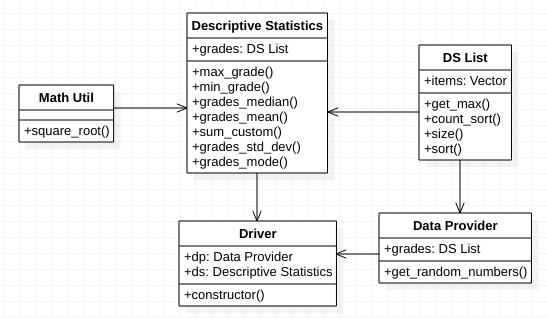
\includegraphics[width=\textwidth]{classdiagram.png}
	\caption{Class Diagram for Descriptive Statistics}
	\label{fig:classdiagram}
\end{figure}

\newpage

\subsection{Weighted Methods per Class}

We can calculate the \gls{wmc} with the following formula:

$$ WMC = \sum\limits_{i=1}^{n} C_{i}(M_{i}) $$ 

where $ C_{i} $ is the complexity of the method $ M_{i} $.\newline

We used the cyclomatic number as a measure of complexity for each method, given that weights are not normalized. Then, using the results found in the section 5, we have:

\begin{equation}
\begin{split}
WMC_{Descriptive Statistics} = C(max\_grade) + C(min\_grade) + C(grades\_median) \\+ C(grades\_mean) + C(sum\_custom) + C(grades\_std\_dev) + C(grades\_mode)
\nonumber
\end{split}
\end{equation}
$$ WMC_{Descriptive Statistics} = 2 + 2 + 2 + 2 + 2 + 5 + 8 $$
$$ WMC_{Descriptive Statistics} = 23 $$

$$ WMC_{DS List} = C(get\_max) + C(count\_sort) + C(size) + C(sort) $$
$$ WMC_{DS List} = 3 + 4 + 1 + 7 $$
$$ WMC_{DS List} = 15 $$

$$ WMC_{Data Provider} =  C(get\_random\_numbers) $$ 
$$ WMC_{Data Provider} = 4 $$

$$ WMC_{Math Util} = C(square\_root) $$ 
$$ WMC_{Math Util} = 3 $$

It does not make sense to calculate the \gls{wmc} for the Driver class since it simply calls functions from the Descriptive Statistics to display the results to the user.

\newpage

\subsection{Coupling Factor}

We can calculate the \gls{cf} using the following formula:

$$ CF = \frac{\sum\limits_{i=1}^{n} \sum\limits_{j=1}^{n} IsClient(C_{i},C_{j})}{n^2-n} $$

$ IsClient(C_{i},C_{j}) $ means that the class $ C_{i} $ has a relationship, either in the form of an attribute or a reference, with the class $ C_{j} $, that is not inheritance.\newline

Based on the diagram above, we have:

$$ CF = \frac{1+1+2+1}{5^2-5} $$
$$ CF = \frac{1}{4} $$

Therefore, the Coupling Factor for Descriptive Statistics is equal to $ \frac{1}{4} $. It is a reasonably low value, meaning that Descriptive Statistics should be analyzable, modifiable and testable. 

\newpage

\subsection{Lack of Cohesion in Methods}

We can calculate the \gls{lcom} using the following formula:

$$ LCOM^{*} = \frac{\frac{1}{a}\sum\limits_{i=1}^{a} \mu(A_{i})-m}{1-m} $$

where $ a $ is the number of attributes, $ m $ the number of methods and $ \mu(A_{k}) $ is the number of methods that access an attribute $ A_{k} $.

We can calculate the \gls{lcom} for each of the classes represented in the class diagram above:

$$ LCOM^{*}_{Descriptive Statistics} = \frac{\frac{1}{1}*(1+1+1+1+1+1)-7}{1-7} $$
$$ LCOM^{*}_{Descriptive Statistics} = \frac{1}{6} $$

$ LCOM^{*}_{Descriptive Statistics} $ is equal to $ \frac{1}{6} $, which a low value, meaning that the Descriptive Statistics class is highly cohesive.

$$ LCOM^{*}_{DS List} = \frac{\frac{1}{1}*(1+1)-4}{1-4} $$
$$ LCOM^{*}_{DS List} = \frac{2}{3} $$

$ LCOM^{*}_{DS List} $ is equal to $ \frac{2}{3} $, which a moderately high value, meaning that the DS List class is slightly cohesive.
\newpage
$$ LCOM^{*}_{Data Provider} = \frac{\frac{1}{1}*(1)-1}{1-1} $$
$$ LCOM^{*}_{Data Provider} = 0 $$

$ LCOM^{*}_{Data Provider} $ is equal to 0 because we used a workaround for the specific case of a class having one method and accessing all of its attributes. This means that there is no lack of cohesion in methods.

$$ LCOM^{*}_{Driver} = \frac{\frac{1}{2}*(1)-1}{1-1} $$
$$ LCOM^{*}_{Driver} = 0 $$

$ LCOM^{*}_{Driver} $ is equal to 0 because we used a workaround for the specific case of a class having one method and accessing all of its attributes. This means that there is no lack of cohesion in methods.

$$ LCOM^{*}_{Math Util} = \frac{\frac{1}{0}*0-1}{1-1} $$
$$ LCOM^{*}_{Math Util} = 0 $$

$ LCOM^{*}_{Math Util} $ is equal to 0 because we used a workaround for the specific case of a class not having any attribute and having one method. This means that there is no lack of cohesion in methods.

Unfortunately, we were not able to find tools that supports R language to calculate those metrics. Such tools exist for Java, but we were unable to find equivalent for R language.

\newpage

\section{LOC}

\subsection{Physical SLOC}

\subsubsection{Manual counting}

We have considered every statement except the blank and commented lines as physical SLOC.

We found the following results:

\begin{table}[ht!]
\centering
\begin{tabular}{|l|l|}
\hline
Source Files              & Physical SLOC \\ \hline
data\_provider.r          & 12            \\ \hline
descriptive\_statistics.r & 83            \\ \hline
driver.r                  & 26            \\ \hline
ds\_list.r                & 44            \\ \hline
math\_util.r              & 17            \\ \hline
Sum                       & 182           \\ \hline
\end{tabular}
\caption{Physical \gls{sloc} count manually}
\end{table}

\subsubsection{Using a tool}

We used \gls{cloc}, an open-source tool written by AlDanial \cite{cloc} and compatible with R to perform the physical \gls{sloc} count. The results for the main classes are as follows:

\begin{figure}[h!]
	\centering
		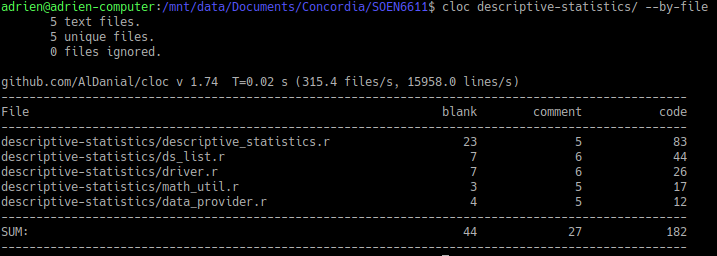
\includegraphics[width=\textwidth]{cloc.png}
	\caption{Physical \gls{sloc} count with CLOC}
	\label{fig:cloc}
\end{figure}

Therefore, the total physical \gls{sloc} for Descriptive Statistics is equal to 182. One can see that we found the same result using the \gls{cloc} tool and manual counting.

\newpage

\subsection{Logical SLOC}

\subsubsection{Manual counting}

We have considered every executable statement, that is the smallest unit of work, as logical SLOC. This means we excluded lines solely composed of a closing parentheses.

We found the following results:

\begin{table}[ht!]
\centering
\begin{tabular}{|l|l|}
\hline
Source Files              & Logical SLOC  \\ \hline
data\_provider.r          & 9            \\ \hline
descriptive\_statistics.r & 63            \\ \hline
driver.r                  & 23            \\ \hline
ds\_list.r                & 33            \\ \hline
math\_util.r              & 13            \\ \hline
Sum                       & 141           \\ \hline
\end{tabular}
\caption{Logical \gls{sloc} count manually}
\end{table}

\subsubsection{Using a tool}

We used SGTools \cite{sgtools}, a collection of R functions written by Sebastian Gibb, that contains a logical \gls{sloc} calculator.

\begin{figure}[h!]
	\centering
		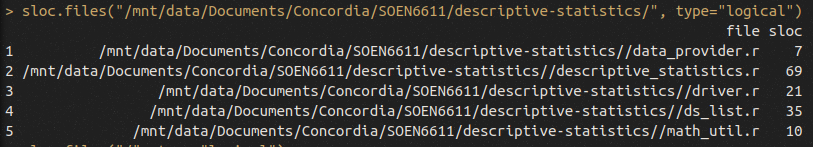
\includegraphics[width=\textwidth]{logicalsloc.png}
	\caption{Logical \gls{sloc} count with SGTools}
	\label{fig:logicalsloc}
\end{figure}

Therefore, the total logical \gls{sloc} for Descriptive Statistics is equal to 142.\newline

\newpage
The difference between the manual and tool calculation is coming from the way we consider closing parentheses: the tool regroups all the closing parentheses in a single line and considers them as one executable statement whereas manual counting does not. Then, it also considers the class declaration and field declaration as a single line. For example, here is how the tool sees the data\_provider class:

\begin{figure}[h!]
	\centering
		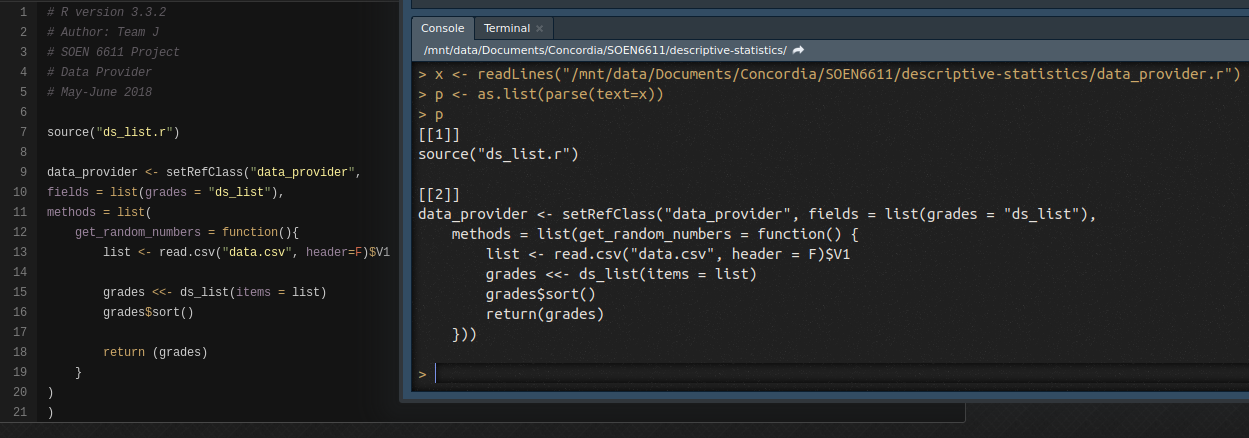
\includegraphics[width=\textwidth]{toolvscode.png}
	\caption{On the left, the actual code for the data\_provider class; on the right, the R script (tool) output for the class}
	\label{fig:toolvscode}
\end{figure}

Counting the number of lines displayed by the tool gives 7 whereas we found 9.

\newpage

\section{Analysis: Correlations between the data for Logical SLOC and WMC}

\subsection{Using Scatter Plot}

\begin{figure}[h!]
	\centering
		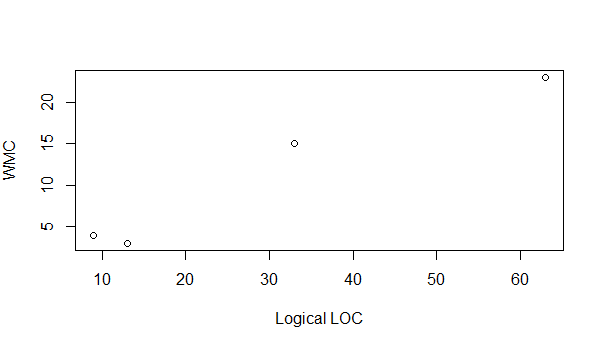
\includegraphics[width=\textwidth]{cor_graph.png}
	\caption{Scatter Plot graph between the logical SLOC and WMC}
	\label{fig:cor_graph}
\end{figure}

From this scatter plot, we can conclude that there is a correlation between the logical SLOC and WMC. As the WMC increases, so does the logical SLOC.

\newpage

\subsection{Using a Correlation Coefficient}

We used the Spearman's rank correlation coefficient to calculate a correlation coefficient between the logical SLOC and WMC.\newline

\begin{table}[ht!]
\centering
\begin{tabular}{|l|l|l|l|l|l|l|}
\hline
Class                   & Logical SLOC & Rank & WMC & Rank & d  & $ d^{2} $ \\ \hline
data\_provider          & 9            & 1    & 4   & 2    & -1 & 1                    \\ \hline
descriptive\_statistics & 63           & 4    & 23  & 4    & 0  & 0                    \\ \hline
ds\_list                & 33           & 3    & 15  & 3    & 0  & 0                    \\ \hline
math\_util              & 13           & 2    & 3   & 1    & 1  & 1                    \\ \hline
\end{tabular}
\caption{A summary of statistics for calculating the $ r_{s} $}
\end{table}

The formula for Spearman's rank correlation is the following:

$$ r_{s} = 1 - \frac{6\sum\limits_{i=1}^{n} d_{i}^{2}}{n^{3} - n} $$ 
$$ r_{s} = 1 - \frac{6\sum\limits_{i=1}^{4} d_{i}^{2}}{4^{3} - 4} $$ 
$$ r_{s} = 1 - \frac{6*(1^{2}+1^{2}+0+0)}{4^{3} - 4} $$
$$ r_{s} = 1 - \frac{12}{60} $$
$$ r_{s} = \frac{4}{5} $$
$$ r_{s} = 0.8 $$

Therefore, we have a positive correlation between the values of the WMC metric and the SLOC of a class.

\newpage

\printglossaries

\newpage

\bibliographystyle{apacite}
\bibliography{references}

\end{document}